\documentclass{beamer}

\usepackage{graphicx}
\usepackage[sfdefault,light]{FiraSans}
%\usefonttheme{serif} 
\usepackage[british]{datetime2}
\usetheme{default}
\setbeamertemplate{navigation symbols}{} % No navigation symbols
\setbeamercolor{alerted text}{fg=blue!80!green!159!}
\setbeamercolor{frame title}{fg=blue!80!green!159!}
\setbeamercolor{title}{fg=blue!80!green!159!}
\setbeamercolor{subtitle}{fg=blue!80!green!159!}
\setbeamercovered{transparent}

\makeatletter
\setbeamertemplate{footline}
{
  \leavevmode%
  \hbox{%
  \begin{beamercolorbox}[wd=.15\paperwidth,ht=2.25ex,dp=1ex,center]{institute in head/foot}%
    \usebeamerfont{title in head/foot}%
    \raisebox{-0.15cm}{
\includegraphics[width=1cm]{logo_ntnu_u-slagord.pdf}}
  \end{beamercolorbox}%
  \begin{beamercolorbox}[wd=.6\paperwidth,ht=2.25ex,dp=1ex,center]{institute in head/foot}%
    \usebeamerfont{title in head/foot}%
    \insertsection
  \end{beamercolorbox}%
  \begin{beamercolorbox}[wd=.15\paperwidth,ht=2.25ex,dp=1ex,center]{institute in head/foot}%
    \usebeamerfont{title in head/foot}%
    \insertshortdate
  \end{beamercolorbox}%
  \begin{beamercolorbox}[wd=.1\paperwidth,ht=2.25ex,dp=1ex,right]{institute in head/foot}%
    \usebeamerfont{title in head/foot} 
    \insertframenumber{} / \inserttotalframenumber\hspace*{2ex} 
  \end{beamercolorbox}}%
}
\makeatother

%----------------------------------------------------------------------------------------
%	TITLE PAGE
%----------------------------------------------------------------------------------------

\title{POL2012: Theories and Models in Political Economy}
\subtitle{Energy politics (climate change)} % Discussion time!
% \date{\today}
\date{}
\author{Marius Swane Wishman}
\institute{Department of Sociology and Political Science}

\begin{document}

\begin{frame}[plain]
\titlepage % Print the title page as the first slide
\centering % Comment out if second logo

\includegraphics[width=5cm]{logo_ntnu_u-slagord.pdf}
%\hspace{0.5cm} 
\includegraphics[width=5cm]{logo_ntnu_u-slagord.pdf} % Second logo
\end{frame}

\section{Energy politics}

\begin{frame}{The political economy of Energy}
\begin{itemize}
    \item Energy $\neq$ electricity \pause
    \begin{itemize}
        \item Different sources for different uses
        \item Fossil fuels \pause
        \item Renewable and non-renewable \pause
    \end{itemize}{}
    \item Technology-economics-politics
    \item Energy and politics
    \item Energy and growth % The importance of vested interests
\end{itemize}{}
\end{frame}{}

\begin{frame}{International politics}
\begin{columns}
\column{0.5\textwidth}
\begin{itemize}
    \item Big money
\end{itemize}{}
\column{0.5\textwidth}
\begin{figure}
    \centering
    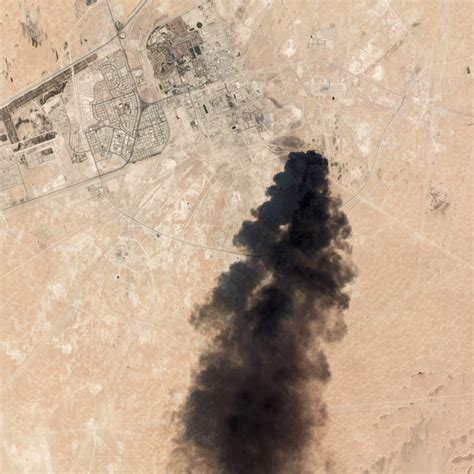
\includegraphics[width=\textwidth]{../img/oilhit.jpg}
\end{figure}
\end{columns}
\end{frame}{}

\begin{frame}{International politics}
\begin{columns}
\column{0.5\textwidth}
\begin{itemize}
    \item Not just big money % Germany 40% of gas from Russia #choke
    % Dams are kind-of like this as well
    \item Energy security
\end{itemize}{}
\column{0.5\textwidth}
\begin{figure}
    \centering
    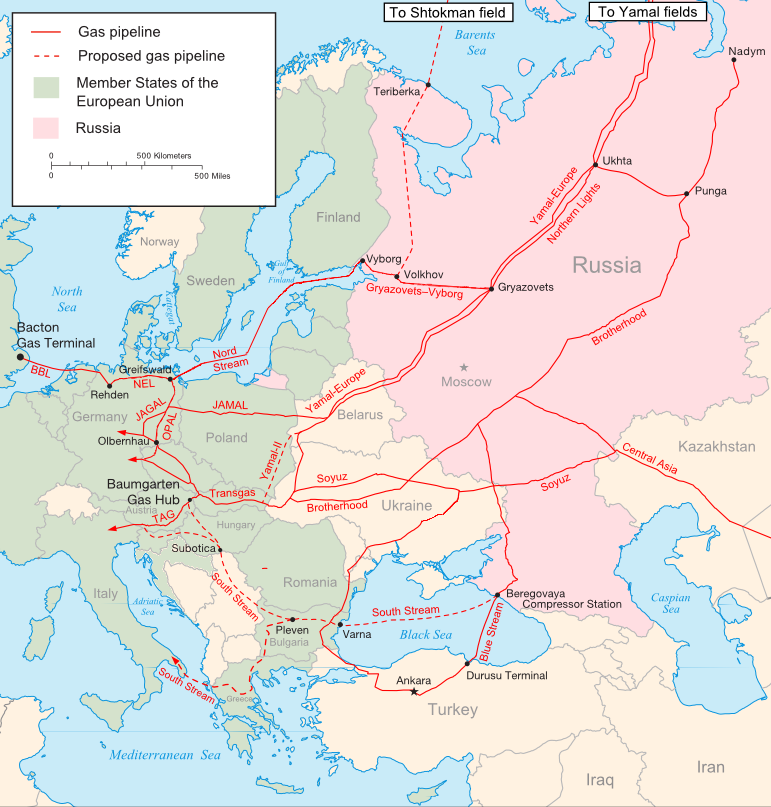
\includegraphics[width=\textwidth]{../img/Major_russian_gas_pipelines_to_europe.png}
\end{figure}
\end{columns}
\end{frame}{}

\begin{frame}{Discuss the statement:}
\centering
    \textit{\Large{``Energy dependence is a source of conflict"}}
\end{frame}{}

\begin{frame}{International politics}
\begin{columns}
\column{0.5\textwidth}
\begin{figure}
    \centering
    
\includegraphics[width=\textwidth]{../img/EU.png}
\end{figure}
\column{0.5\textwidth}
\begin{figure}
    \centering
    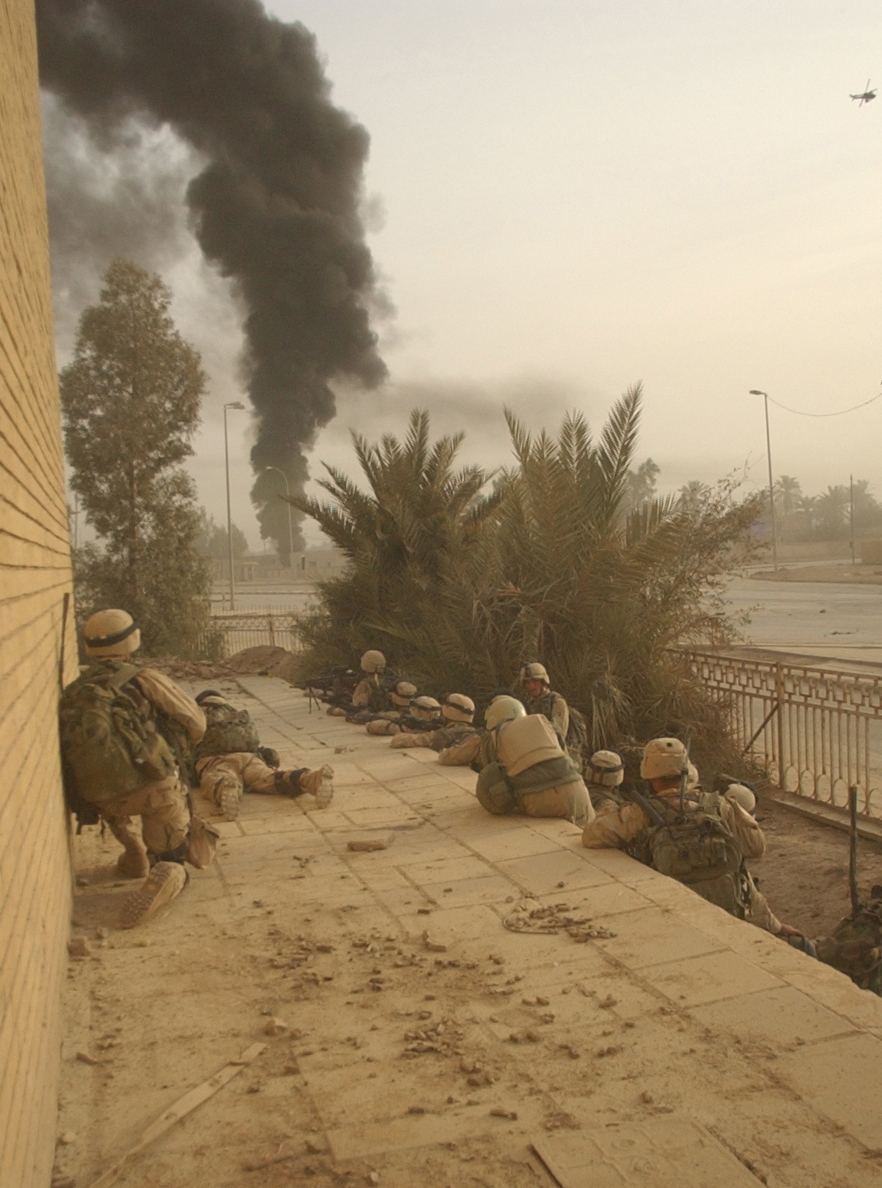
\includegraphics[width=\textwidth]{../img/USinvasion.jpg}
\end{figure}
\end{columns}
\end{frame}{}

\section{Climate change}

\begin{frame}{Climate change}
\begin{figure}
    \centering
    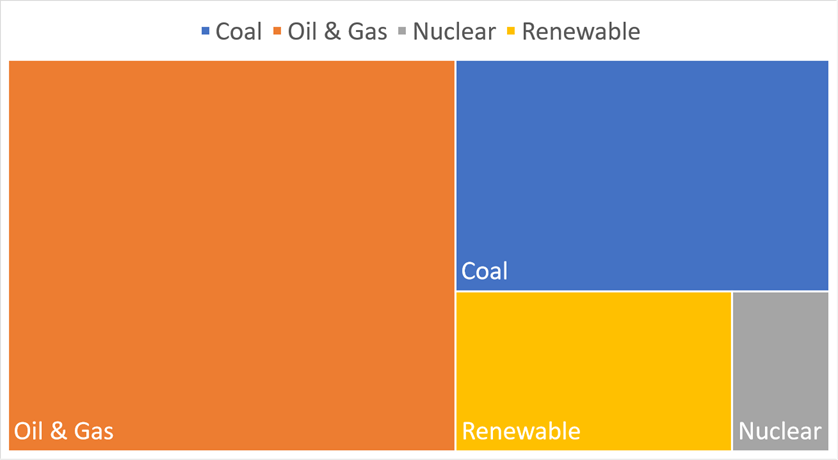
\includegraphics[width=\textwidth]{../img/energy.png}
    \caption{Current global energy supply}
\end{figure}
\end{frame}{}

\begin{frame}{What needs to happen?}
\begin{itemize}
    \item Change the type of energy used \pause
    \item Change source of electricity \pause % most electricity is still produced by coal, gas second
    \item How do they interact? % # Thanks Marshall!
\end{itemize}{}
\end{frame}{}

\begin{frame}{The problem of the grid}
\begin{figure}[htpb]
	\centering
	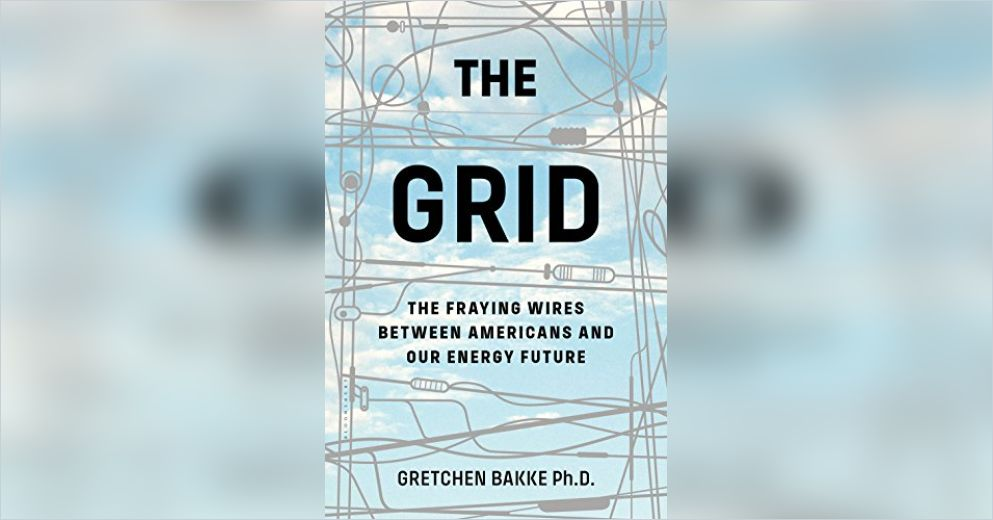
\includegraphics[width=0.8\linewidth]{../img/grid.jpeg}
\end{figure}
\end{frame}

\begin{frame}{The problem of the grid}
\begin{figure}[htpb]
	\centering
	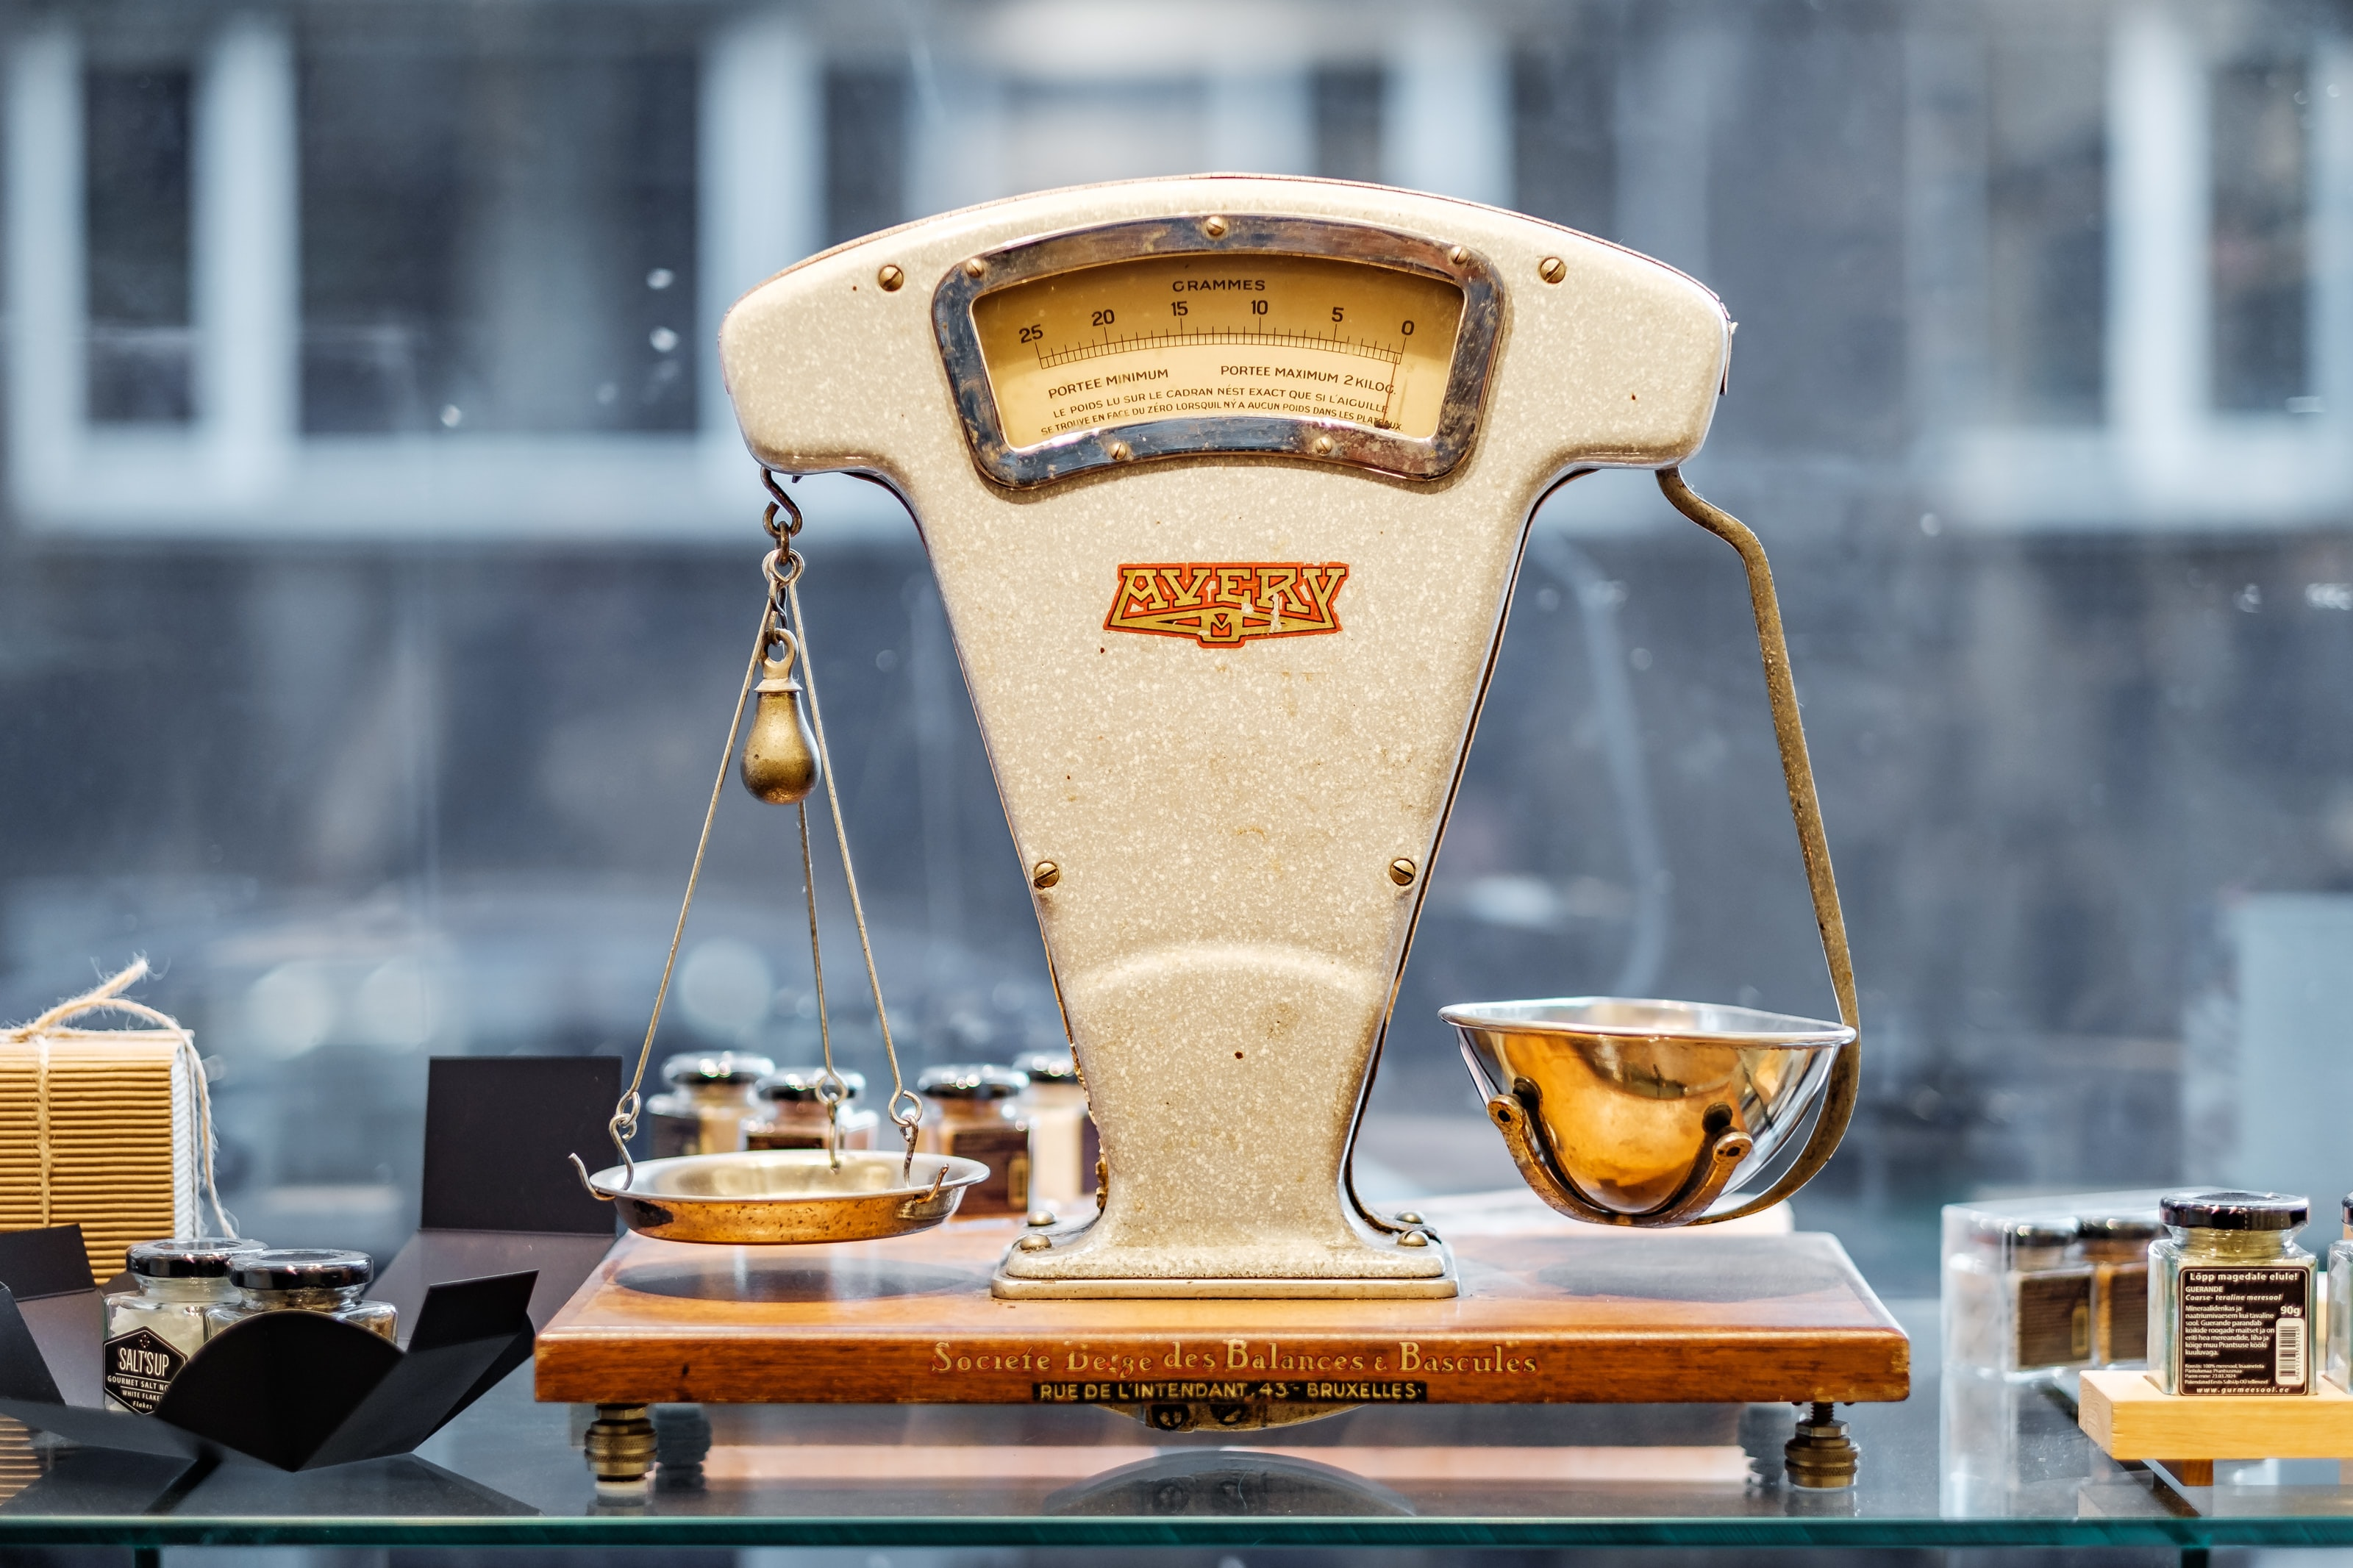
\includegraphics[width=0.8\textwidth]{../img/balance.jpg}
\end{figure}
\end{frame}

\section{The Green Shift}

\begin{frame}{Market mechanisms} % Short of revolution, this is pretty much what we got
% Fiat is an option, but seems even more unlikely
\begin{itemize}
    \item Make renewable energy competitive \pause
    \item Carbon taxes and ETS
\end{itemize}{}
\end{frame}{}

\begin{frame}{}
\centering
\textit{\Large{Alternatives to the market?}} % ARGUMENTS!
\end{frame}{}

\begin{frame}{}
\centering
\textit{\Large{Will it work?}} % ARGUMENTS!
\end{frame}{}

\begin{frame}{Potential problems}
\begin{itemize}
    \item Vested interests \pause
    \item Energy systems are built around fossil fuels \pause 
    \item Energy efficiency \pause
    % Energy efficiency is an alternative to structural/system change
    % Cost effective, make a plane use less fuel > make an electric plane
    % Good, but not enough?
    \item Only works if our assumptions hold % What is the cheapest source of energy? Clean/not-clean?
\end{itemize}{}
\end{frame}{}

\begin{frame}{}
\begin{figure}
    \centering
    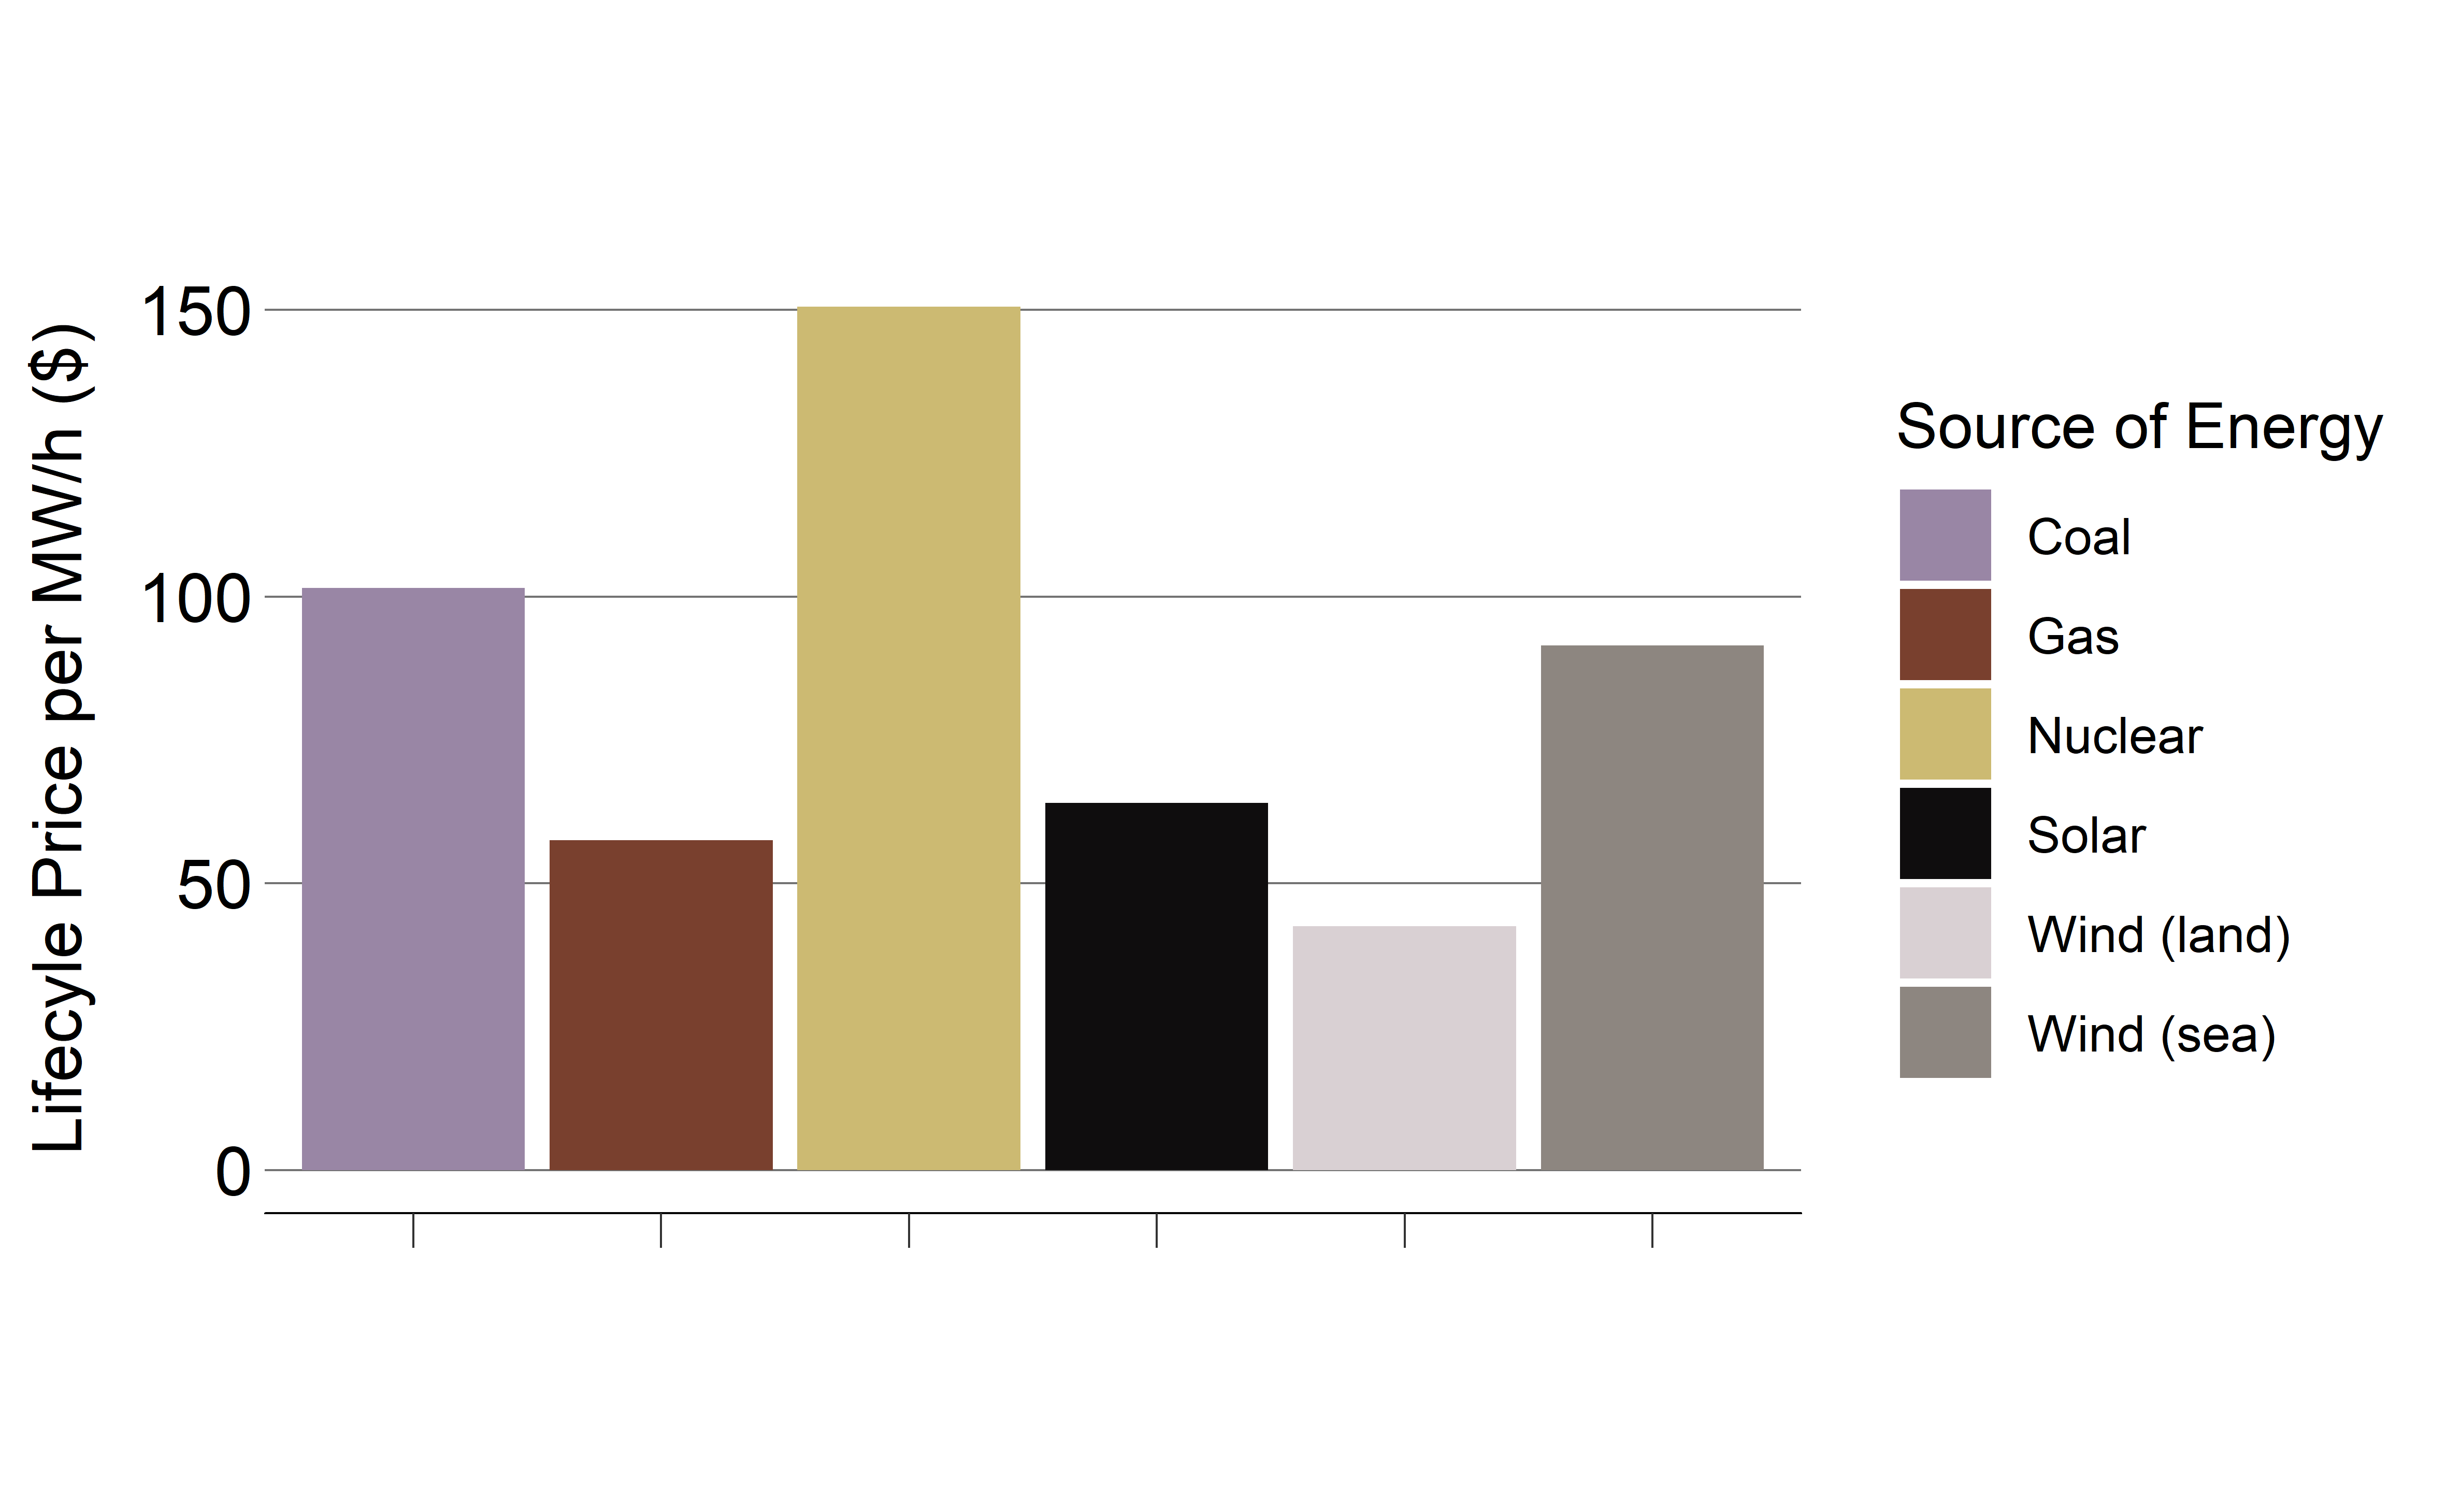
\includegraphics[width=\textwidth]{../img/Electric.png}
\end{figure}{}
\end{frame}{}

\end{document} 


